\documentclass[a4paper, 12pt]{article}%тип документа

%отступы
\usepackage[left=2cm,right=2cm,top=2cm,bottom=3cm,bindingoffset=0cm]{geometry}

%Русский язык
\usepackage[T2A]{fontenc} %кодировка
\usepackage[utf8]{inputenc} %кодировка исходного кода
\usepackage[english,russian]{babel} %локализация и переносы

%Вставка картинок
\usepackage{graphicx}
\graphicspath{{pictures/}}
\DeclareGraphicsExtensions{.pdf,.png,.jpg}

%Графики
\usepackage{multirow}
\usepackage{pgfplots}
\pgfplotsset{compat=1.9}

%Римские цифры
\newcommand{\RNumb}[1]{\uppercase\expandafter{\romannumeral #1\relax}}

%Математика
\usepackage{amsmath, amsfonts, amssymb, amsthm, mathtools}

%Красная строка
\usepackage{indentfirst}
\parindent=1cm

%Цвет текста
\usepackage{color}

%Заголовок
\author{Богданов Александр \\
	Б05-003}
\title{\textbf{Закон Мозли}}

\begin{document}

\maketitle

    \section*{Аннотация}

		Я решил сделать лабораторную работу - закон Мозли.  Этот закон показывает зависимость энергии излучаемого атомом рентгеновского кванта при переходе электрона с оболочки одного слоя на другой от заряда атома. 
	
		Я выбрал именно эту работу,  так как Закон Мозли является доказательством правильности размещения элементов в периодической системе элементов Д. И. Менделеева и содействует выяснению физического смысла $Z$.  А также из-за того,  что данная закономерность лежит в основе рентгенофлуоресцентного анализа,  позволяющего определять элементный состав образцов.

    \section*{Цель работы}

		Измерить спектры характеристического излучения атомов для набора химических элементов.  Определить рентгеновские термы измеренных спектральных пиков излучения.  Проверить закон Мозли.

    \section*{В работе используется}

		Рентгеновский спектрометр <<Спектроскан Макс-G>>,  компьютер,  образцы чистых химических элементов.
		
    \section*{Теоретические сведения}
		
		\textbf{Электронные состояния атома}\\
	
		Энергетический спектр состояний электрона в атоме водорода имеет вид:

		\[E_n = -\frac{me^4}{2\hbar^2} \frac{1}{n^2} = -Ry \frac{1}{n^2}, \]
			
		Строгий учёт спина у электрона возможен при решении задачи об атоме водорода с помощью релятивистского уравнения Дирака.  Наличие спина у электрона приводит к возникновению спин-орбитального взаимодействия.  Важным результатом такого взаимодействия является то,  что электрон в состоянии,  соответствующем заданному уровню энергии,  также обладает определённым полным моментом импульса $j$.  То есть энергия состояния оказывается зависящей не только от главного квантового числа $n$,  но и от величины полного момента $j$, что приводит к тонкому расщеплению уровней энергии. 

		Электронные состояния,  определяемые парой чисел $(n,  l)$,  называются электронной оболочкой,  среднее расстояние между электронном и ядром зависит от этих чисел:

		\[< r >_{n,  l} = \frac{r_{\text{Б}}}{2} (3n^2 - l(l + 1))\]
			
где $r_{\text{Б}}$ – боровский радиус. 

		Атомы химических элементов,  отличных от водорода,  включают в себя более чем один электрон,  и их описание возможно только приближёнными методами,  поскольку электроны взаимодействуют не только с ядром атома,  но и друг с другом.   Так,  если описывать некоторый многоэлектронный атом,  пренебрегая взаимодействием между электронами и не учитывая спин электронов,  то для каждого электрона в отдельности получится система энергетических уровней,  описываемых формулой:

		\[E_n = - \frac{me^4}{2\hbar^2} \frac{Z^2}{n^2} = -Ry \frac{Z^2}{n^2}, \]
			
		Полученный таким способом результат для многоэлектронного атома не даёт количественного согласия с экспериментальными данными,  поскольку межэлектронное взаимодействие вносит существенный вклад.  Для уточнения этой модели необходимо учесть межэлектронное,  спинорбитальное и другие типы взаимодействий.  Межэлектронное электростатическое взаимодействие оказывает наиболее существенное влияние на величину энергетических уровней,  поэтому рассмотрим этот фактор подробнее.

		Приближённо учёт электростатического межэлектронного взаимодействия можно провести следующим образом.  Для заданного электрона,  находящегося в некотором состоянии (n,  l,  m),  суммарное действие всех других электронов,  в основном сводится к частичному экранированию заряда ядра.  Величина этого экранирования зависит от количества электронов,  средние радиусы оболочек которых меньше либо равны радиусу оболочки (nl).  Можно ввести константу экранирования $\sigma_{n, l}$,  так что формула примет вид:

		\[E_{n,  l} = -\frac{me^4}{2\hbar^2} \frac{(Z - \sigma_{n, l})^2}{n^2} = -Ry \frac{(Z - \sigma_{n, l})^2}{n^2}\]
			
		Для электронов,  находящихся в состояниях,  локализованных близко к ядру,  эта формула хорошо описывает основной вклад в энергию их взаимодействия с атомом.\\
				
		\textbf{Излучательные переходы и рентгеновские термы}\\
				
		Основное состояние атома -- состояние с наименьшей энергией.  При этом,  в согласии с правилом запрета Паули,  заполнены все электронные состояния,  начиная с самого <<глубокого>> и до некоторого валентного состояния.  Если в таком атоме некоторый электрон перейдёт в какое-то другое свободное электронное состояние,  то атом окажется в возбуждённом состоянии.  Такой переход может сопровождаться испусканием фотона.  При этом,  должны сохраняться энергия и момент импульса.  При рассмотрении процессов излучения и поглощения фотонов, сопровождающихся только перестройкой электронных оболочек,  спин ядра можно считать неизменным.  Поэтому в дальнейшем полагаем, что момент импульса атома равен суммарному моменту импульса всех его электронов.
   
		Момент импульса каждой полностью заполненной электронной оболочки $(nl)$ равен нулю.  Поэтому момент импульса атома определяется только моментом незаполненных электронных оболочек. 
								
		Нас будут интересовать переходы между возбуждёнными состояниями атома,  обусловленные переходами электронов между различными состояниями с малыми значениями главного квантового числа $n$.  Для возможности таких переходов необходимо наличие свободного электронного состояния на глубоком уровне.  Освободить состояние можно за счёт поглощения фотона с достаточно большой энергией. Уровни энергии атома,  у которого удалён один из электронов с глубокого уровня,  называют рентгеновскими термами.  Энергия рентгеновского терма зависит не только от числа $n$,  но и от момента $j$ электронной оболочки с вакансией.  Для рентгеновских термов система обозначений: 
				
		\begin{figure}[h!]
			\centering
			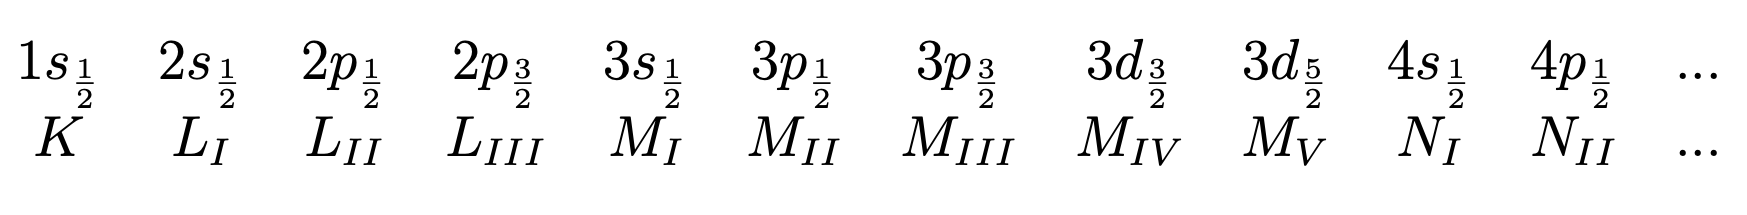
\includegraphics[scale=0.5]{Рентгеновские_термы.png}
			\caption{Обозначения рентгеновских термов}
		\end{figure}
				
		\textbf{	Характеристическое излучение и закон Мозли}\\

		При переходе электрона с оболочки одного слоя на другой слой атом излучает рентгеновский квант,  такое излучение называется характеристическим излучением.  Энергия кванта такого излучения приближённо может быть записана в виде:
			
		\[\hbar \omega_{1,2} = - Ry \left( \frac{(Z - \sigma_{n_2,  l_2})^2}{n_2^2} - \frac{(Z - \sigma_{n_2,  l_2})^2}{n_1^2} \right)\]

		Или

		\[\hbar \omega = Ry (Z - \sigma)^2 \left( \frac{1}{n_1^2} - \frac{1}{n_2^2}\right)\]

		Основным подтверждением формулы является хорошее совпадение с экспериментом.  
				
		Из-за расщепления рентгеновских термов спектр излучения каждой серии будет состоять из нескольких близких компонент. 

		\begin{figure}[h!]
			\centering
			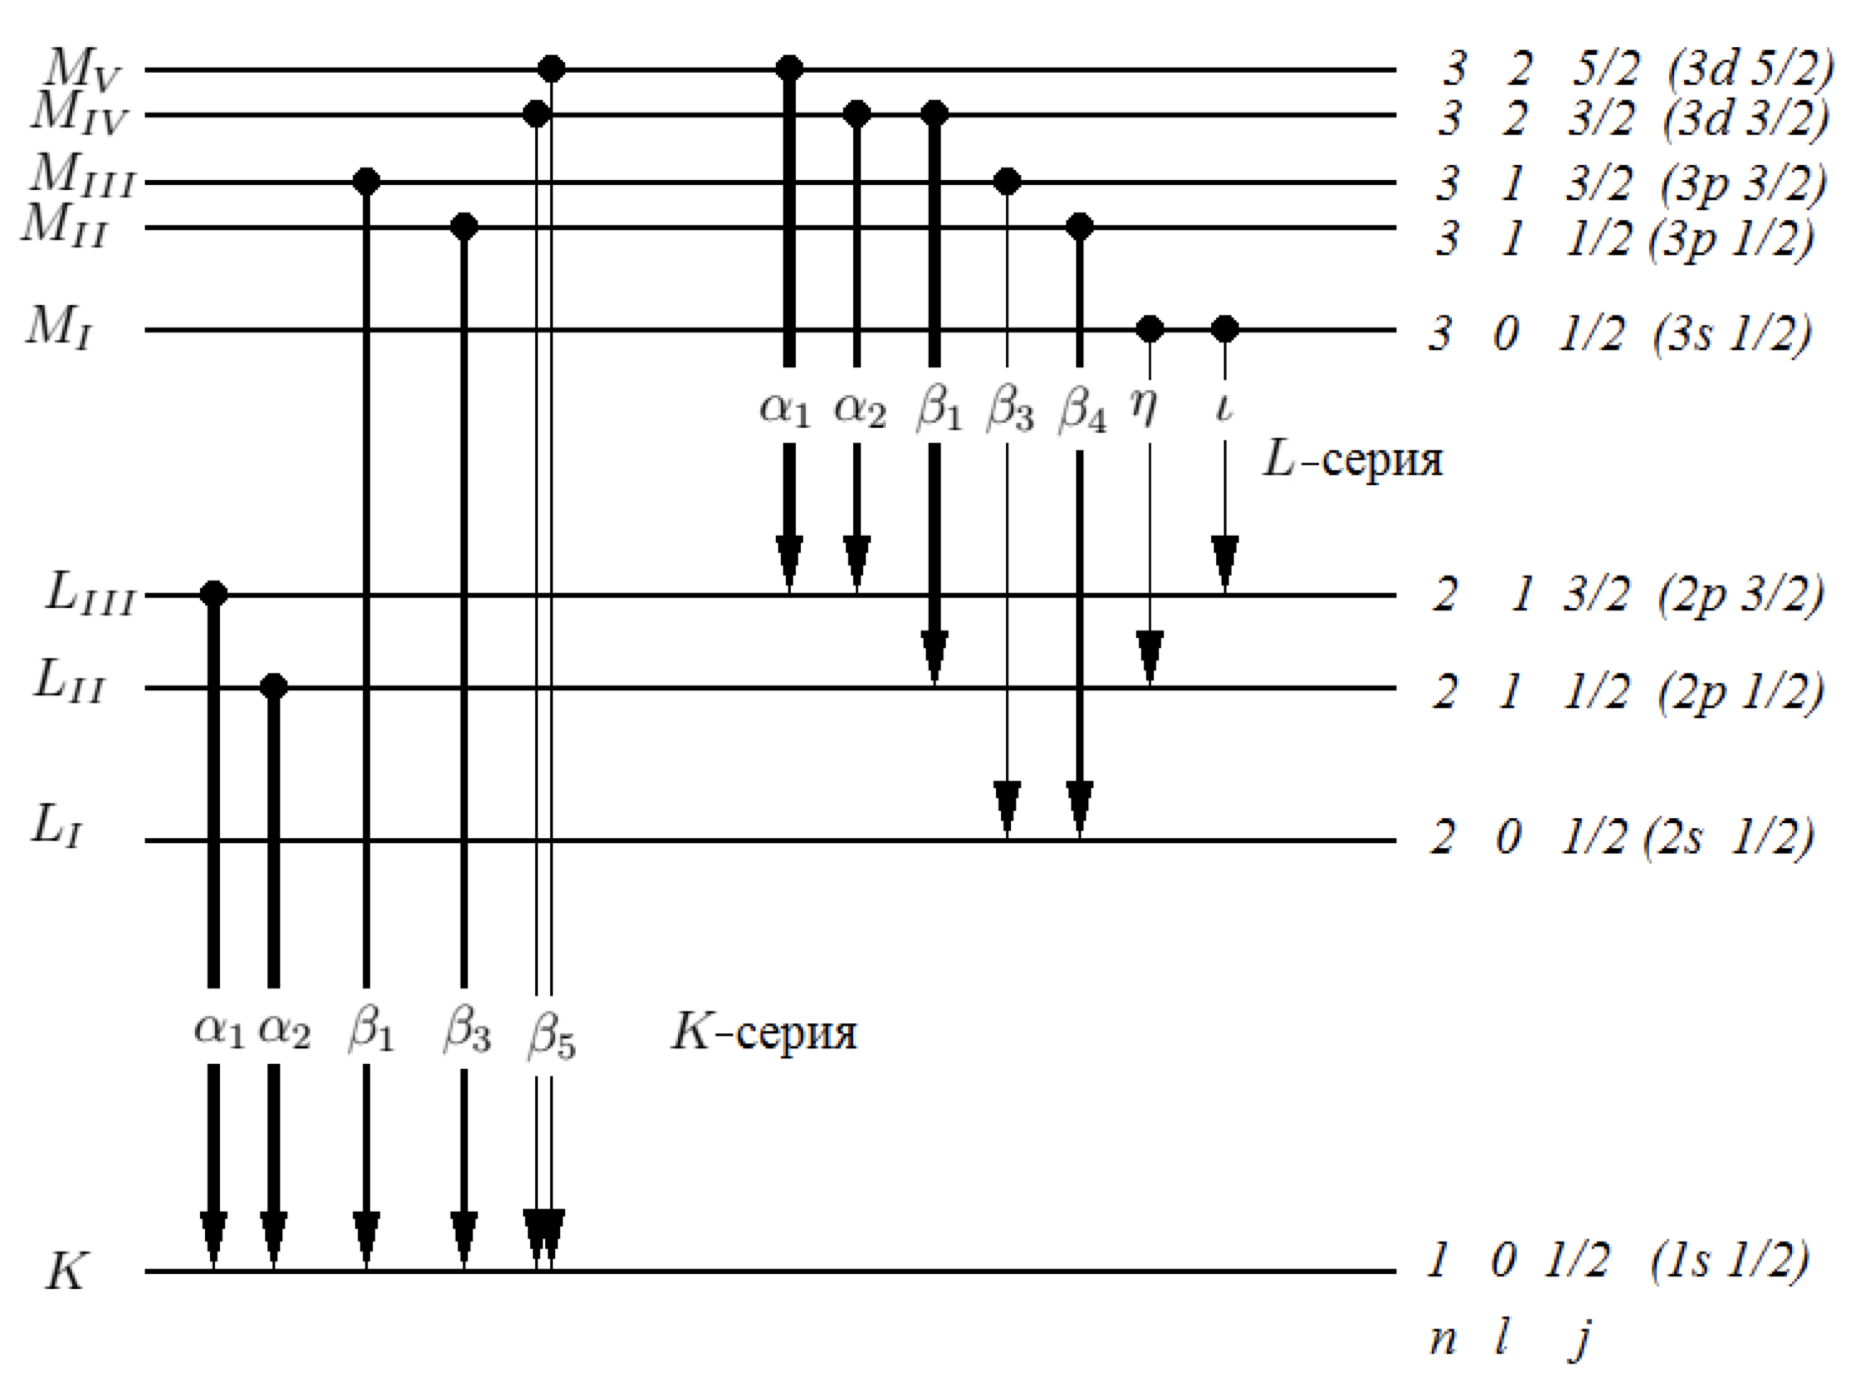
\includegraphics[scale=0.35]{Переходы.png}
			\caption{Переходы K-серии и L-серии}
		\end{figure}

	\newpage

    \section*{Экспериментальная установка}
		
		\textbf{Устройство рентгеновского спектрометра}\\
			
		Для регистрации рентгеновских спектров характеристического излучения в работе используется рентгенофлуоресцентный спектрометр <<Спектроскан Макс-G>>. 
				
		\begin{figure}[h!]
			\centering
			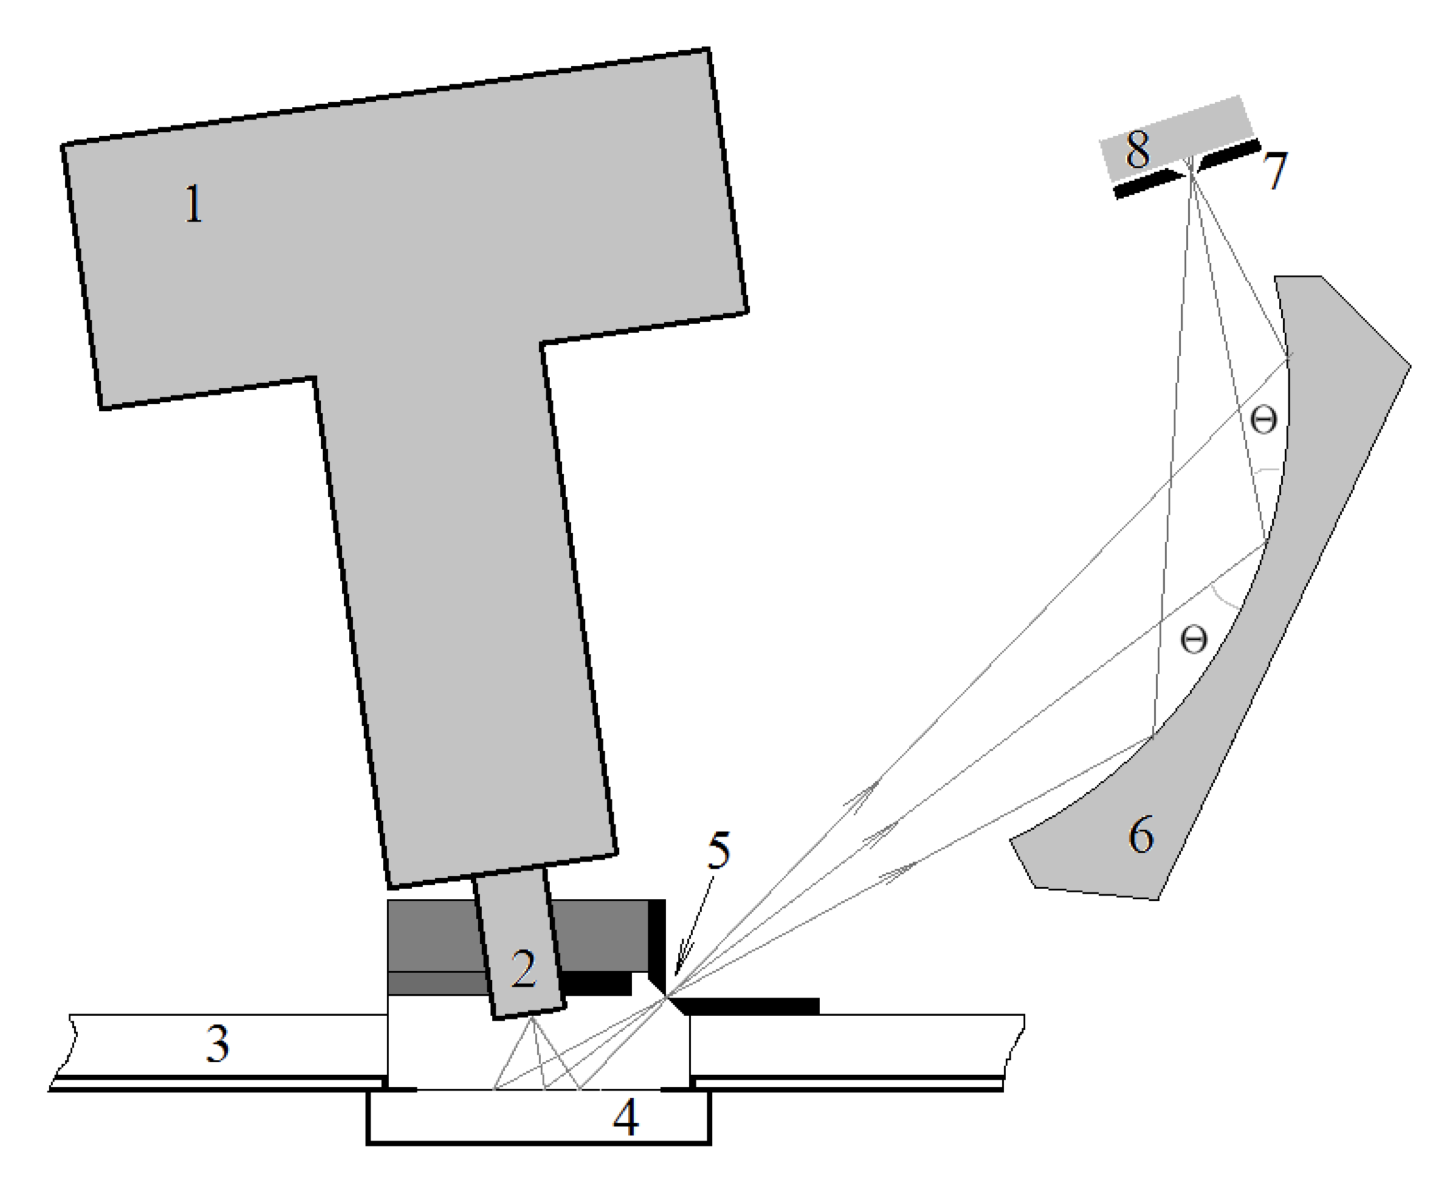
\includegraphics[scale=0.45]{Схема_установки.png}
			\caption{Схема рентгеновского спектрометра}
		\end{figure}				
				
		В состав спектрометра входят следующие основные элементы: 
				
		\begin{enumerate}
				
			\item Рентгеновский трубка
					
			\item Носик рентгеновской трубки
					
			\item Основное днище прибора
		
			\item Образец
					
			\item Щель
		
			\item Дифракционное зеркало
			
			\item Щель
					
			\item Пропорциональный детектор
		
		\end{enumerate}
				
		Рентгеновская трубка 1 установлена так,  что её носик 2 с выходным окном располагается непосредственно над поверхностью анализируемого образца 4.  Образец подаётся ниже основного днища прибора 3 с помощью специального механизма.  
				
		Рентгеновское излучение образуется за счёт торможения разогнанных электронов в тонком слое меди,  которая нанесена на бериллиевую пластинку,  прозрачную для рентгеновских лучей.  Непрерывное тормозное излучение трубки <<освещает>> на поверхности образца небольшую область.  Под воздействием этого излучения происходит возбуждение атомных элементов,  которые при релаксации испускают характеристическое излучение.  
				
		Часть этого излучения через щель 5 попадает на изогнутую поверхность кристалла LiF -- дифракционного зеркала 6.  Кристалл представляет собой тонкую пластинку,  приклеенную к изогнутой металлической поверхности.  Отражение от зеркала может претерпевать только излучение с определённой длиной волны,  которая определяется условием дифракции Брэгга-Вульфа и зависит от угла $\theta$ падения рентгеновских лучей на пластину. 
				
		Отразившееся излучение попадает через щель 7 в пропорциональный детектор 8,  с помощью которого производиться регистрация рентгеновских квантов и оценочное определение их энергии.  С помощью специальной электро-механической системы реализован гониометр - прибор для высокоточного измерения углов,  который позволят,  последовательно перемещая зеркало и детектор излучения,  менять значения угла дифракции $\theta$. 
				
		Применение изогнутого кристалла позволяет увеличить <<оптическую силу>> схемы,  направить больше излучения на детектор,  что в свою очередь позволяет снизить необходимую мощность рентгеновской трубки и повысить уровень радиационной безопасности прибора.  
				
		Излучение от источника,  расположенного на фокальной окружности радиуса $R$ и отражающееся от вогнутого зеркала с радиусом $2R$,  снова сфокусируется на той же окружности,  которая называется фокальным кругом Роуланда.  
				
		\begin{figure}[h!]
			\centering
			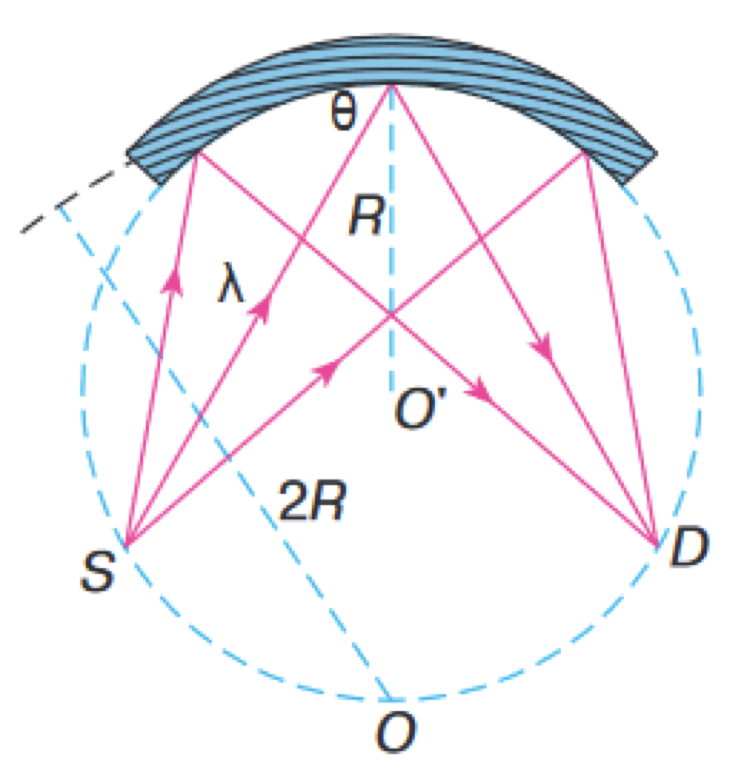
\includegraphics[scale=0.5]{Круг_Роуланда.png}
			\caption{Отражение по схеме Иоганссона}
		\end{figure}				
				
		В приборе используется дифракционное отражение от вогнутой пластинки LiF по схеме Иоганссона. Тонкую монокристаллическую пластинку LiF предварительно отшлифовывают так, чтобы он приобрела цилиндрическую форму радиуса $2R$,  а атомные слои оставались плоскими.  Затем эту заготовку наклеивают на цилиндрическую поверхность радиуса $R$.  В результате изгиба атомные слои,  выполняющие функцию зеркала,  приобретают кривизну радиуса $2R$,  так что вогнутая поверхность пластинки становиться частью круга Роуланда.  В приборе щель-источник 5 и щель-приёмник 7 детектора при любых углах отражения остаются расположенными на фокальном круге Роуланда.  Такая схема позволяет сфокусировать рентгеновское излучение на детекторе и повысить <<оптическую>> силу прибора.	
				
		Для регистрации квантов излучения используется газоразрядный детектор.  Он выполнен в виде герметично запаянного цилиндра 1,  который наполнен инертным газом.  Вдоль оси цилиндра натянута тонкая металлическая нить-анод 2,  изолированная от корпуса.  Внутренняя сторона корпуса выполнена из проводящего материала и представляет собой цилиндрический катод.  Между нитью и катодом подаётся высокое напряжение.  В боковой стенке корпуса сделано узкое бериллиевое окно 3, через которое рентгеновское излучение попадает в детектор.  Рентгеновский квант,  попадая в объём газа детектора, ионизирует некоторое количество атомов газа.  Образовавшиеся свободные электроны под действием электрического поля ускоряются и,  сталкиваясь с другими атомами,  выбивают новые электроны – происходит лавинообразное увеличение числа электронов,  котрые формируют импульс тока через детектор. 
				
		\begin{figure}[h!]
			\centering
			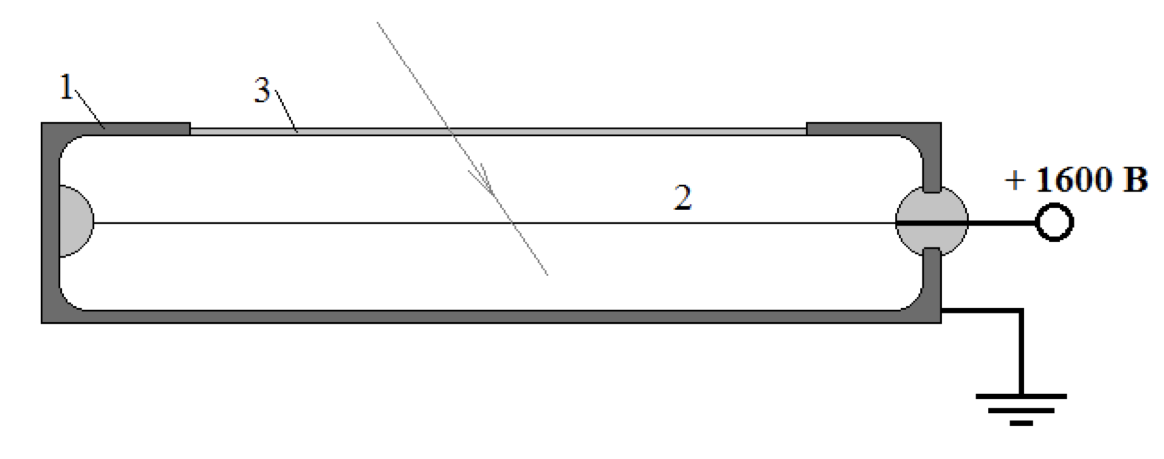
\includegraphics[scale=0.5]{Схема_детектора.png}
			\caption{Схема газоразрядного детектора}
		\end{figure}					
				
		Особенностью работы детектора,  установленного в спектрометре,  является ступенчатый характер зависимости амплитуды выходных импульсов от энергии рентгеновских квантов.  Такой режим работы детектора позволяет соотносить импульсы малой амплитуды с излучением,  отражённым в первом порядке дифракции,  а импульсы с высокой амплитудой – с излучением отражённым во втором порядке дифракции. 	

		Таким образом,  базовый метод определения энергии рентгеновских квантов основан на явлении дифракции Брэгга-Вульфа,  а спектральная чувствительность пропорционального детектора используется для различения первого и второго порядков дифракции.\\
			
		\textbf{Программное обеспечение спектрометра}\\
			
		Управление спектрометром осуществляется через компьютер с использованием специального комплекса программ.
					
    \section*{Ход работы}

		В лабораторной работе мы определили длины волн характеристического излучения следующих элементов: $^{23}$V,  $^{27}$Co,  $^{28}$Ni,  $^{34}$Se, $^{39}$Y,  $^{42}$Mo,  $^{47}$Ag,  $^{49}$In,  $^{57}$La,  $^{62}$Sm,  $^{67}$Ho, $^{72}$Hf,  $^{74}$W,  $^{76}$Os,  $^{80}$Hg,  $^{82}$Pb.

		Работали мы с наиболее яркими спектральными линиями,  а именно: $K_{\alpha_{1, 2}},  K_{\beta_{1, 3}},  L_{\alpha_1}$ и $L_{\beta_1}$.  При этом указанные линии $K$-серии мы определяли для первой половины перечисленных элементов: от ванадия до индия включительно,  а линии $L$-серии -- для второй половины: от лантана до свинца.

		При обработке нового образца запускаем быстрое <<измерение спектра>>, а затем качественно промеряем два наибольших пика,  так как исследуемые нами линии обладают наибольшей интенсивностью.

		Приведем спектры всех элементов, которые мы измеряли.  На этих рисунках красными отмечены экспериментальные точки,  а синим цветом выделены наиболее яркие спектральные линии.

		\begin{figure}[h]
			\begin{minipage}[h]{0.49\textwidth}
				\begin{center}
					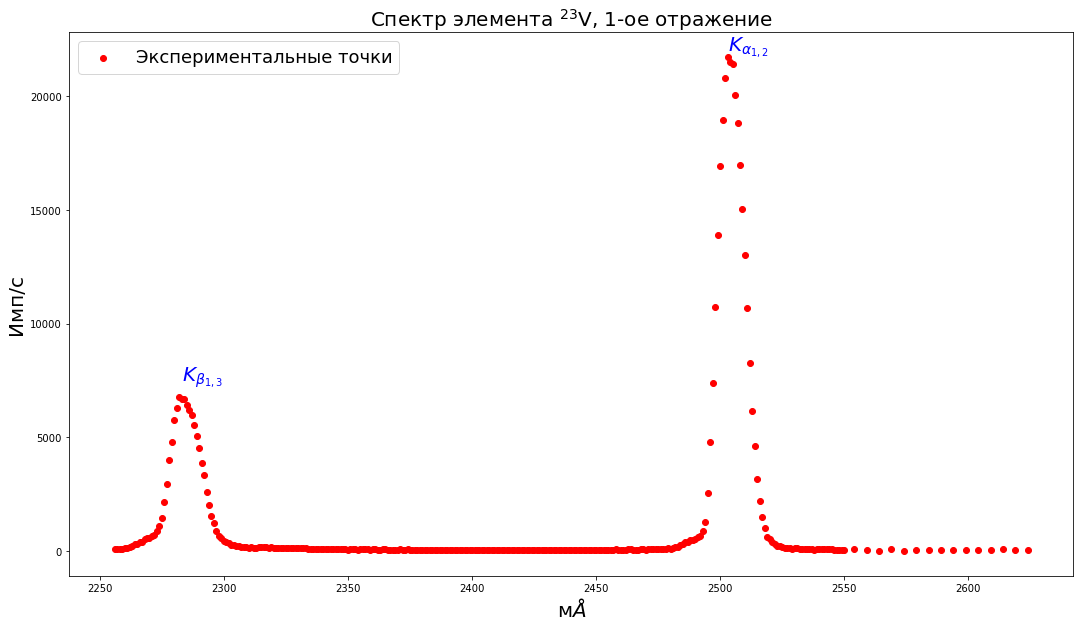
\includegraphics[width=1.02\linewidth]{Спектры/V.png}
					\caption{Спектр $^{23}$V}
				\end{center}
			\end{minipage}
			\hfill
			\begin{minipage}[h]{0.49\textwidth}
				\begin{center}
					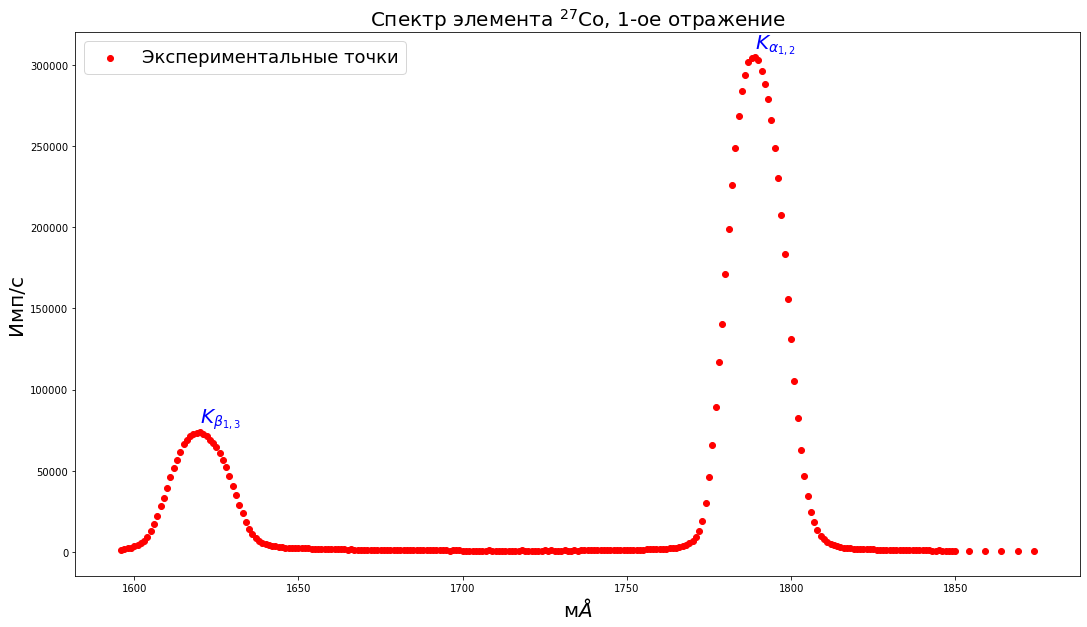
\includegraphics[width=1.02\linewidth]{Спектры/Co.png}
					\caption{Спектр $^{27}$Co}
			\end{center}
			\end{minipage}
		\end{figure}

	\newpage

		\begin{figure}[h]
			\begin{minipage}[h]{0.49\textwidth}
				\begin{center}
					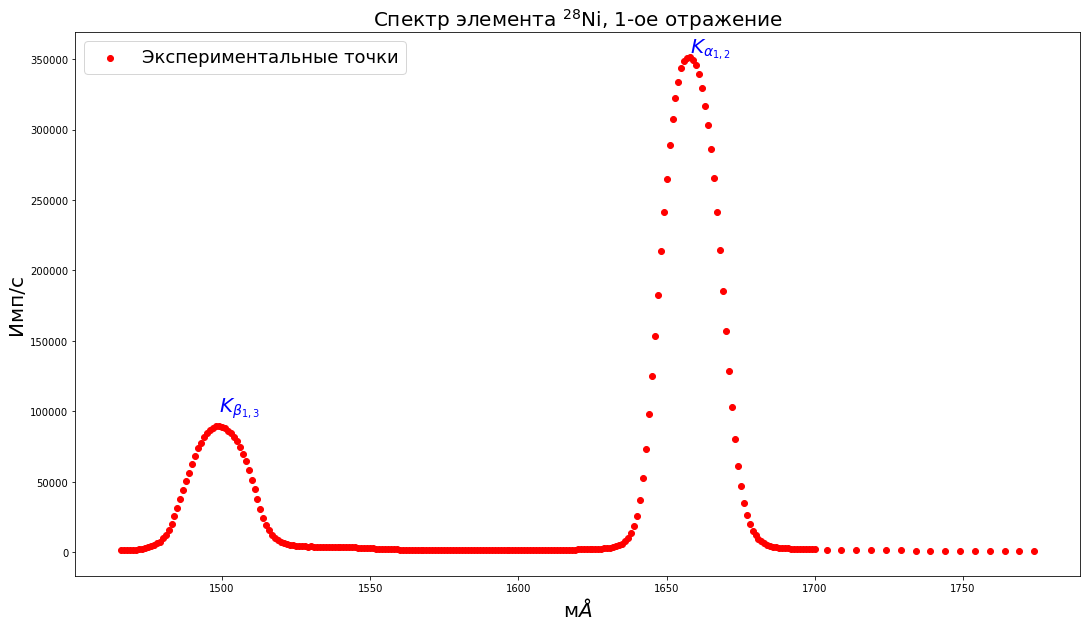
\includegraphics[width=1.02\linewidth]{Спектры/Ni.png}
					\caption{Спектр $^{28}$Ni}
				\end{center}
			\end{minipage}
			\hfill
			\begin{minipage}[h]{0.49\textwidth}
				\begin{center}
					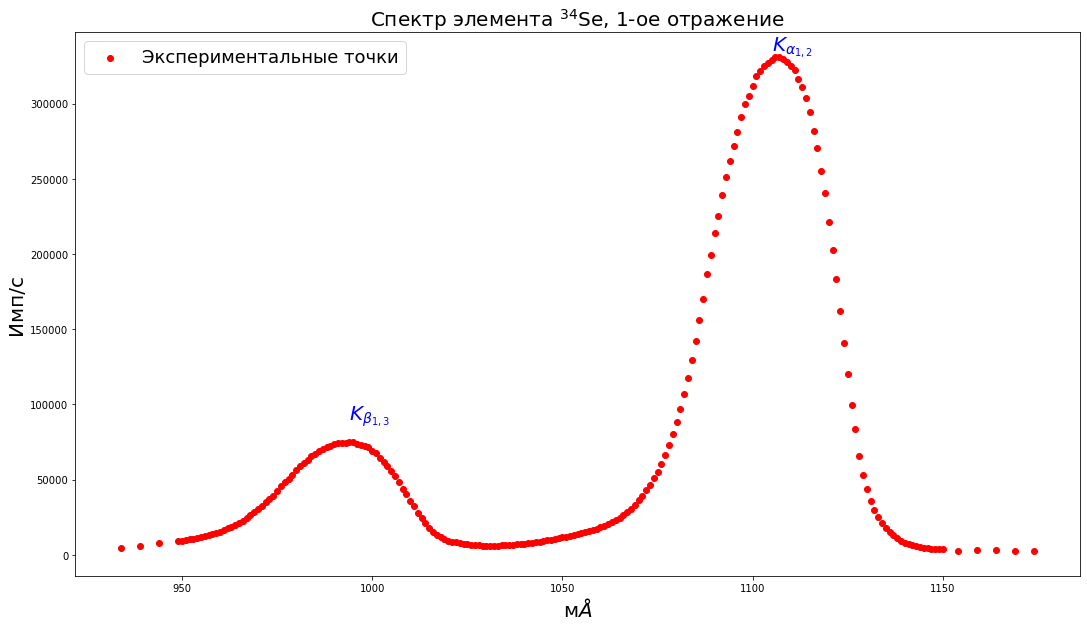
\includegraphics[width=1.02\linewidth]{Спектры/Se.png}
					\caption{Спектр $^{34}$Se}
				\end{center}
			\end{minipage}
		\end{figure}

		\begin{figure}[h!]
			\begin{minipage}[h]{0.49\textwidth}
				\begin{center}
					\includegraphics[width=1.02\linewidth]{Спектры/y.png}
					\caption{Спектр $^{39}$Y}
				\end{center}
			\end{minipage}
			\hfill
			\begin{minipage}[h]{0.49\textwidth}
				\begin{center}
					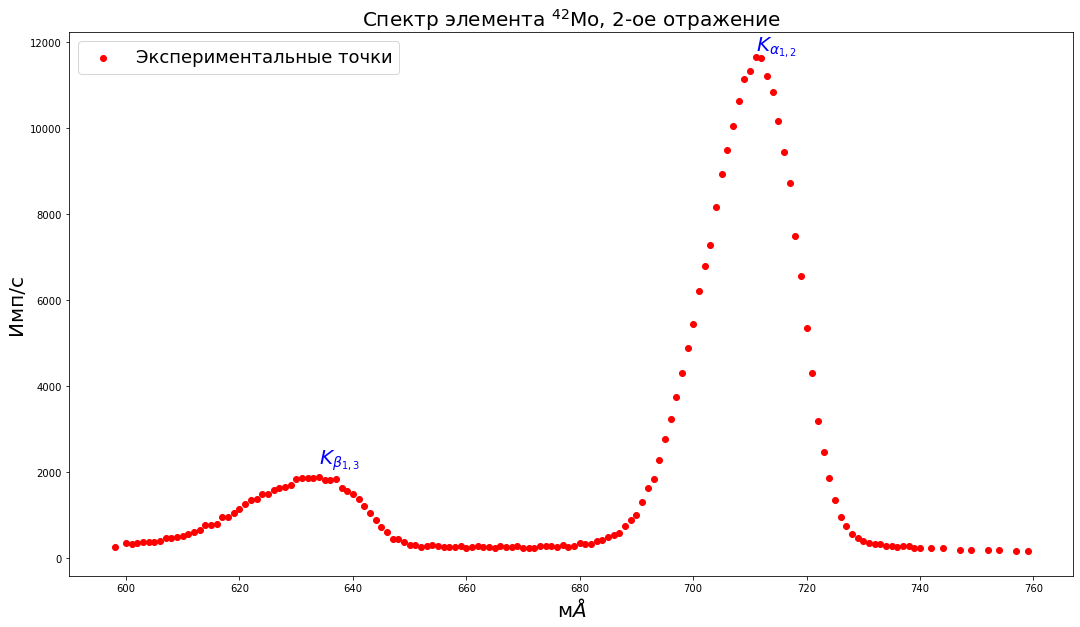
\includegraphics[width=1.02\linewidth]{Спектры/Mo.png}
					\caption{Спектр $^{42}$Mo}
				\end{center}
			\end{minipage}
		\end{figure}

		\begin{figure}[h!]
			\begin{minipage}[h]{0.49\textwidth}
				\begin{center}
					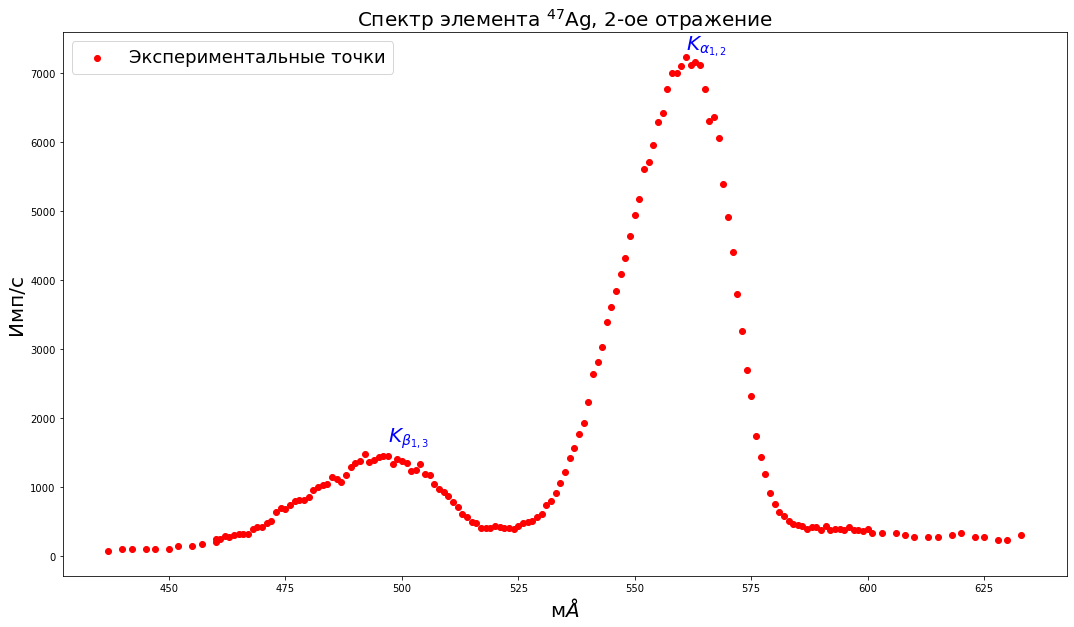
\includegraphics[width=1.02\linewidth]{Спектры/Ag.png}
					\caption{Спектр $^{47}$Ag}
				\end{center}
			\end{minipage}
			\hfill
			\begin{minipage}[h]{0.49\textwidth}
				\begin{center}
					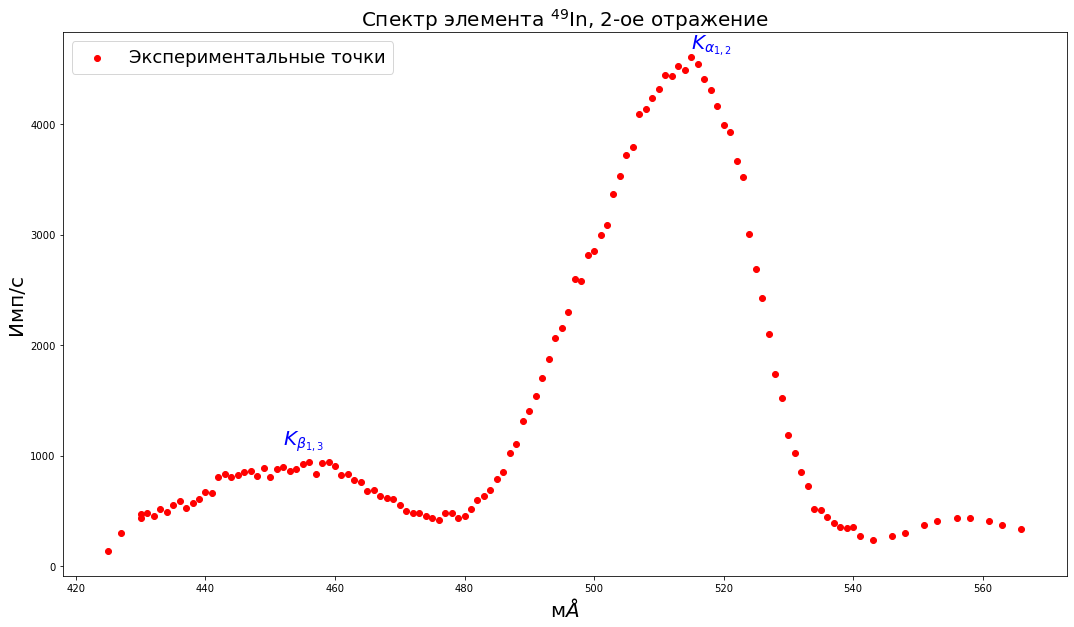
\includegraphics[width=1.02\linewidth]{Спектры/In.png}
					\caption{Спектр $^{49}$In}
				\end{center}
			\end{minipage}
		\end{figure}

		\newpage

		\begin{figure}[h!]
			\begin{minipage}[h]{0.49\textwidth}
				\begin{center}
					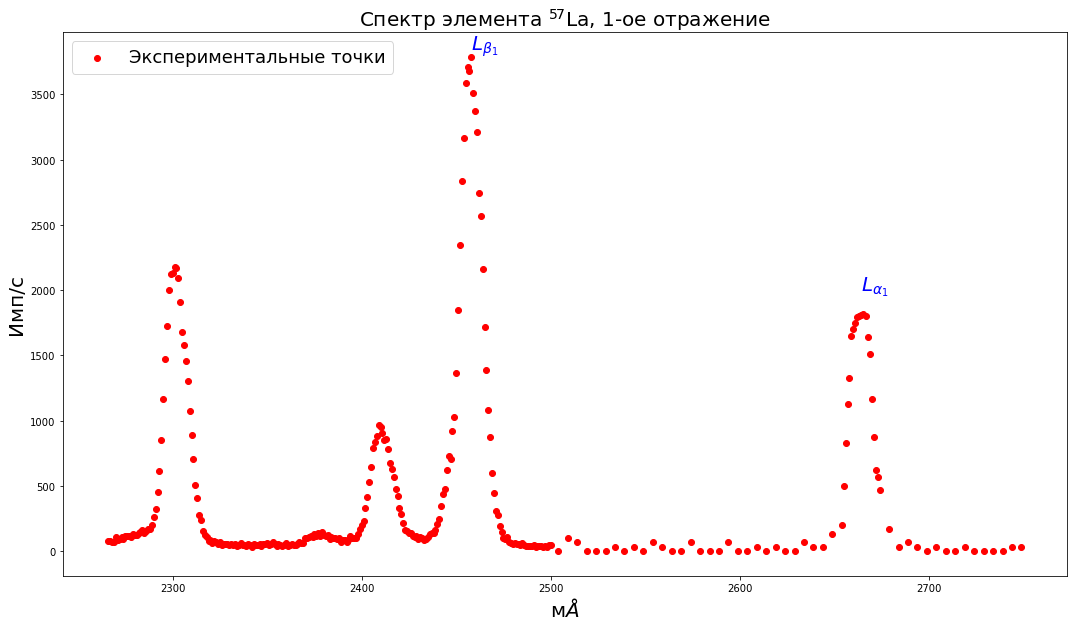
\includegraphics[width=1.02\linewidth]{Спектры/La.png}
					\caption{Спектр $^{57}$La}
				\end{center}
			\end{minipage}
			\hfill
			\begin{minipage}[h]{0.49\textwidth}
				\begin{center}
					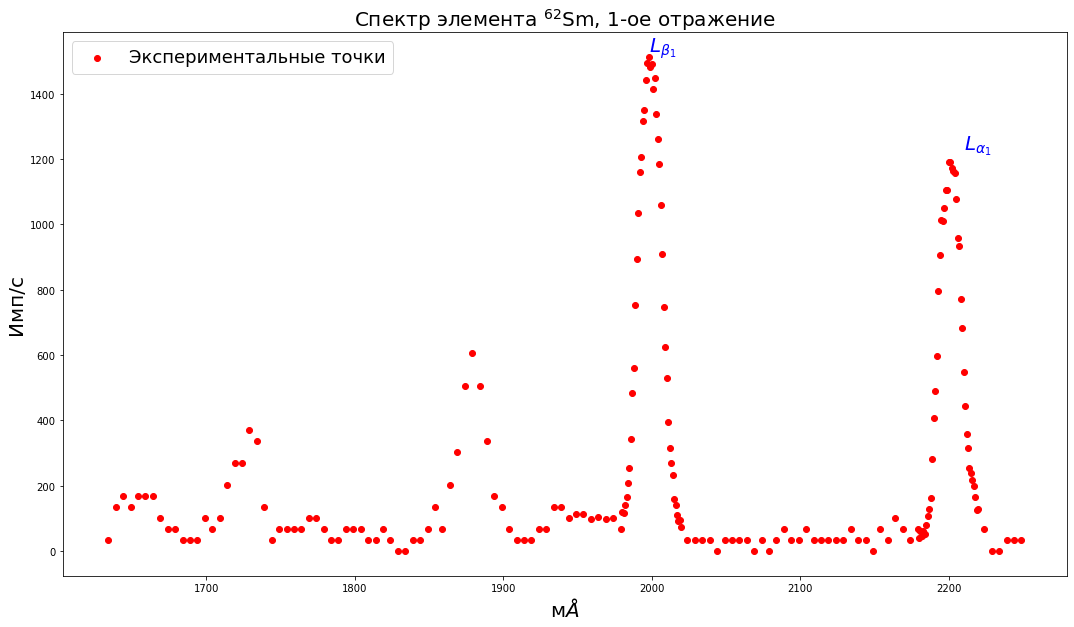
\includegraphics[width=1.02\linewidth]{Спектры/Sm.png}
					\caption{Спектр $^{62}$Sm}
				\end{center}
			\end{minipage}
		\end{figure}

		\begin{figure}[h!]
			\begin{minipage}[h]{0.49\textwidth}
				\begin{center}
					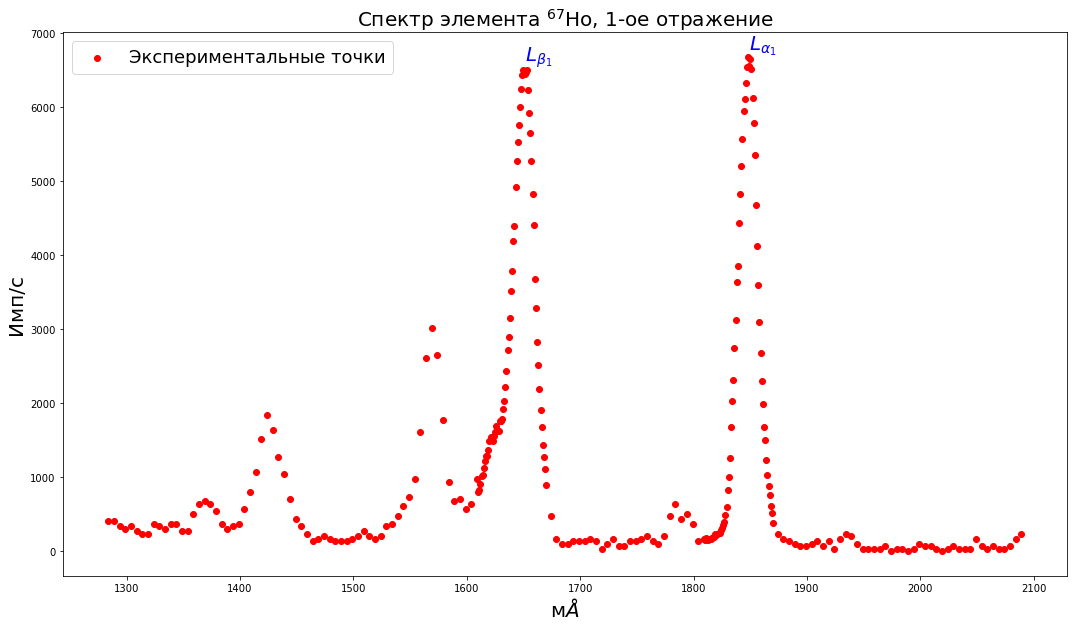
\includegraphics[width=1.02\linewidth]{Спектры/Ho.png}
					\caption{Спектр $^{67}$Ho}
				\end{center}
			\end{minipage}
			\hfill
			\begin{minipage}[h]{0.49\textwidth}
				\begin{center}
					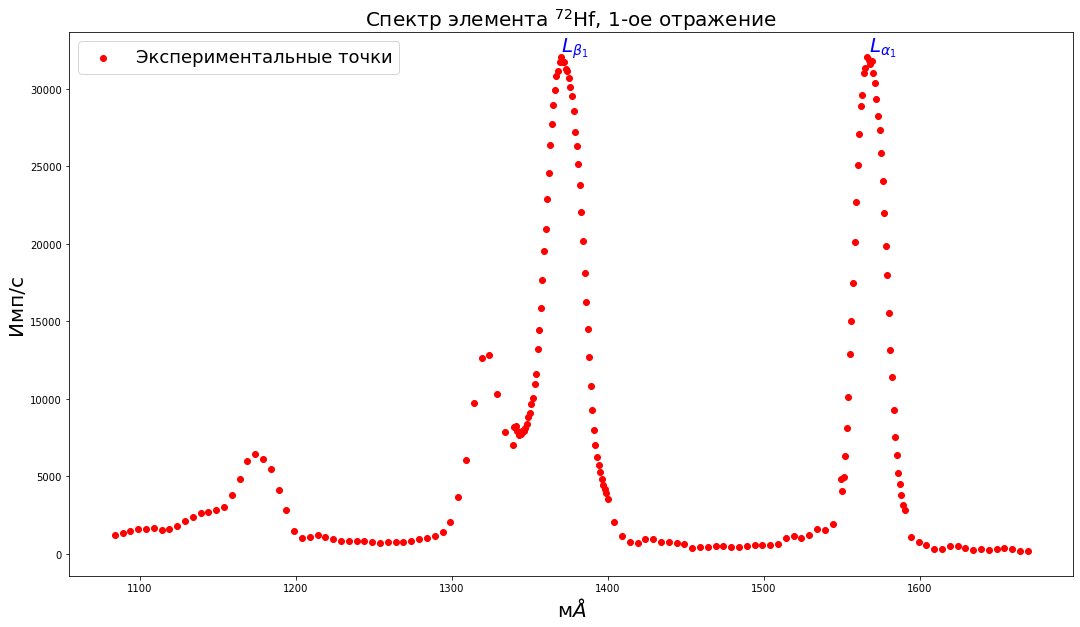
\includegraphics[width=1.02\linewidth]{Спектры/Hf.png}
					\caption{Спектр $^{72}$Hf}
				\end{center}
			\end{minipage}
		\end{figure}

		\begin{figure}[h!]
			\begin{minipage}[h]{0.49\textwidth}
				\begin{center}
					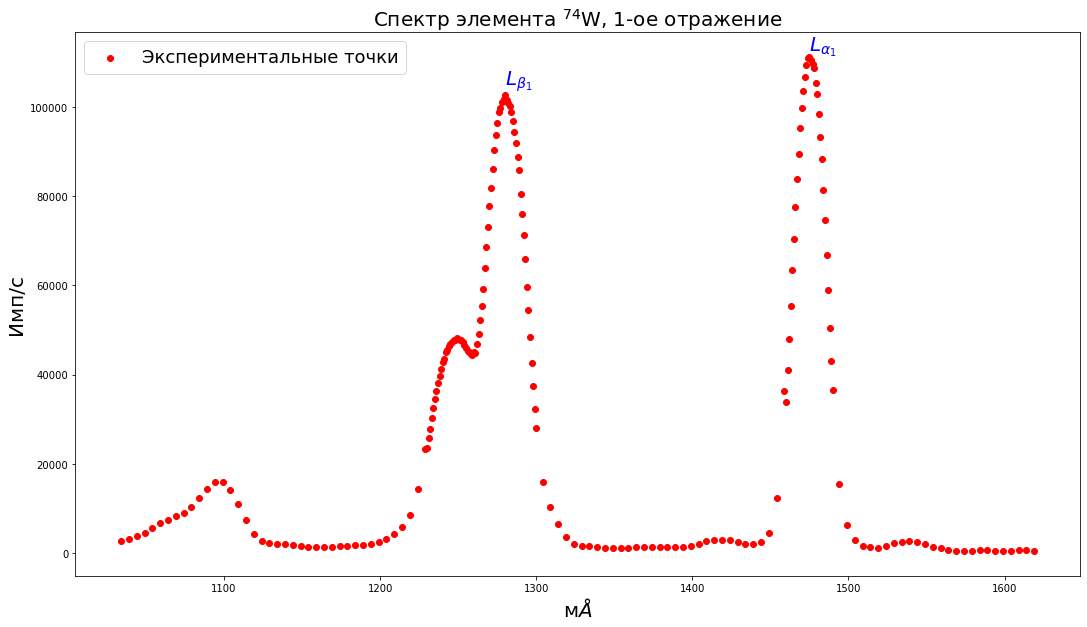
\includegraphics[width=1.02\linewidth]{Спектры/W.png}
					\caption{Спектр $^{74}$W}
				\end{center}
			\end{minipage}
			\hfill
			\begin{minipage}[h]{0.49\textwidth}
				\begin{center}
					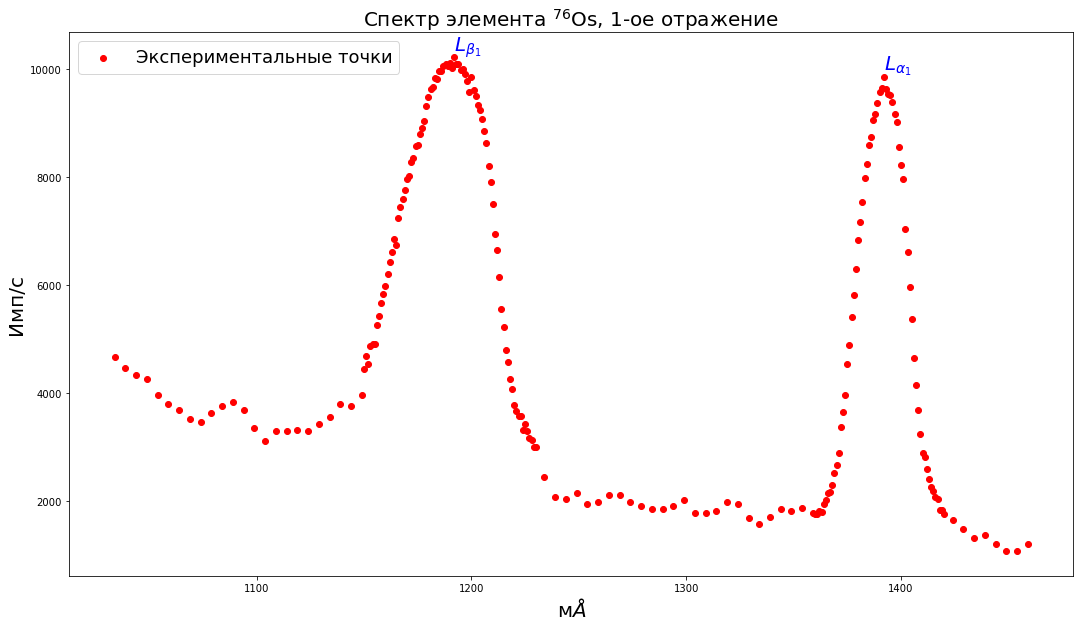
\includegraphics[width=1.02\linewidth]{Спектры/Os.png}
					\caption{Спектр $^{76}$Os}
				\end{center}
			\end{minipage}
		\end{figure}

		\newpage

		\begin{figure}[h!]
			\begin{minipage}[h]{0.49\textwidth}
				\begin{center}
					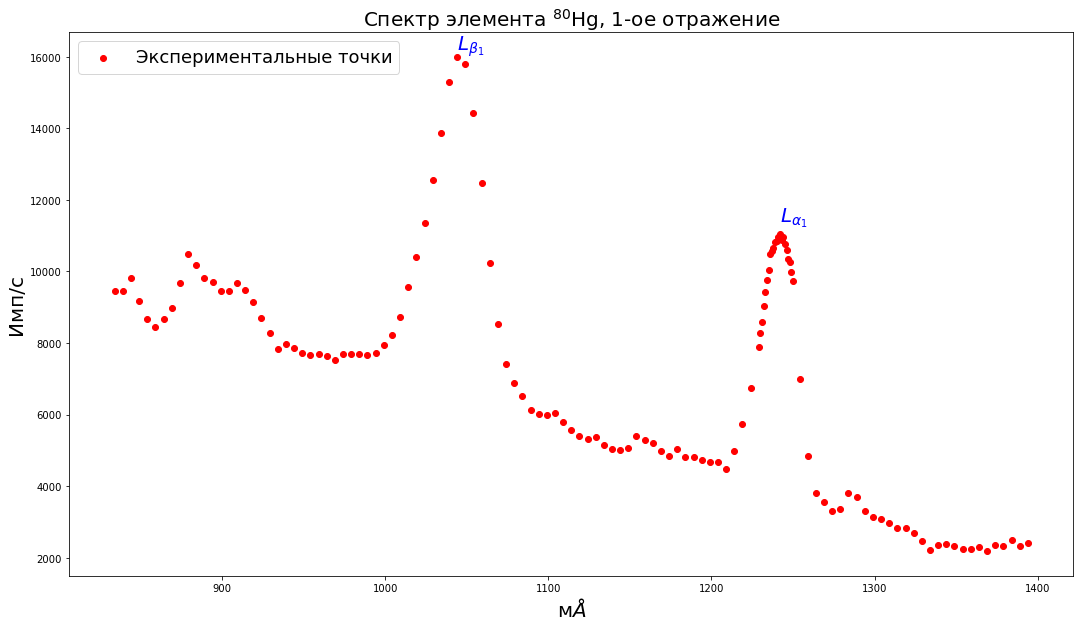
\includegraphics[width=1.02\linewidth]{Спектры/Hg.png}
					\caption{Спектр $^{80}$Hg}
				\end{center}
			\end{minipage}
			\hfill
			\begin{minipage}[h]{0.49\textwidth}
				\begin{center}
					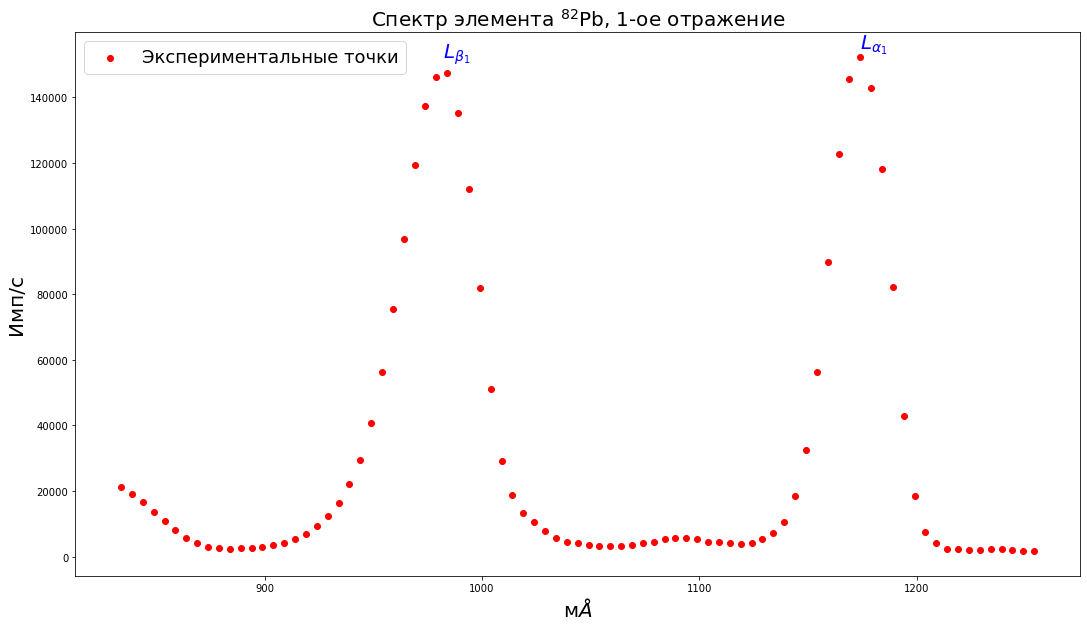
\includegraphics[width=1.02\linewidth]{Спектры/Pb.png}
					\caption{Спектр $^{82}$Pb}
				\end{center}
			\end{minipage}
		\end{figure}

	На основании измеренных данных получим:

		\begin{table}[!ht]
    			\centering
			\begin{tabular}{|c|c|c|c|c|c|c|c|c|c|}
				\hline
				Хим. & $Z$ & $\lambda_{K_{\alpha}}$,  м\AA & $\lambda_{K_{\beta}}$,  м\AA & $E_{K_{\alpha}}$,  Эв & $E_{K_{\beta}}$,  Эв & $\sqrt{\frac{E_{K_{\alpha}}}{R_y}}$ & $\sigma\left(\sqrt{\frac{E_{K_{\alpha}}}{R_y}}\right)$ & $\sqrt{\frac{E_{K_{\beta}}}{R_y}}$ & $\sigma\left(\sqrt{\frac{E_{K_{\beta}}}{R_y}}\right)$  \\
				\hline
				V & 23 & 2503 & 2283 & 4957 & 5435 & 19.088 & 0.005 & 19.987 & 0.004 \\ 
				Co & 27 & 1789 & 1620 & 6936 & 7660 & 22.579 & 0.008 & 23.728 & 0.007 \\ 
				Ni & 28 & 1658 & 1499 & 7484 & 8277 & 23.453 & 0.009 & 24.665 & 0.008 \\ 
				Se & 34 & 1105 & 994 & 11228 & 12483 & 28.728 & 0.016 & 30.290 & 0.015 \\ 
				Y & 39 & 829 & 740 & 14967 & 16767 & 33.168 & 0.025 & 35.106 & 0.024 \\ 
				Mo & 42 & 711 & 634 & 17451 & 19571 & 35.815 & 0.032 & 37.928 & 0.030 \\ 
				Ag & 47 & 561 & 497 & 22117 & 24965 & 40.320 & 0.046 & 42.837 & 0.043 \\ 
				In & 49 & 515 & 452 & 24093 & 27451 & 42.082 & 0.053 & 44.919 & 0.050 \\
				\hline
			\end{tabular}
			\caption{Результаты измерений для легких элементов}
		\end{table}

		\begin{table}[!ht]
			\centering
			\begin{tabular}{|c|c|c|c|c|c|c|c|c|c|}
				\hline
				Хим. & $Z$ & $\lambda_{L_{\beta}}$,  м\AA & $\lambda_{L_{\alpha}}$,  м\AA & $E_{L_{\beta}}$,  Эв & $E_{L_{\alpha}}$,  Эв & $\sqrt{\frac{E_{L_{\beta}}}{R_y}}$ & $\sigma\left(\sqrt{\frac{E_{L_{\beta}}}{R_y}}\right)$ & $\sqrt{\frac{E_{L_{\alpha}}}{R_y}}$ & $\sigma\left(\sqrt{\frac{E_{L_{\alpha}}}{R_y}}\right)$  \\
				\hline
				La & 57 & 2458 & 2664 & 5048 & 4658 & 19.262 & 0.003 & 18.503 & 0.003 \\ 
				Sm & 62 & 1998 & 2201 & 6210 & 5637 & 21.365 & 0.004 & 20.356 & 0.005 \\ 
				Ho & 67 & 1651 & 1849 & 7515 & 6711 & 23.503 & 0.006 & 22.209 & 0.006 \\ 
				Hf & 72 & 1370 & 1567 & 9057 & 7918 & 25.801 & 0.007 & 24.125 & 0.008 \\ 
				W & 74 & 1280 & 1475 & 9694 & 8412 & 26.693 & 0.008 & 24.866 & 0.008 \\ 
				Os & 76 & 1192 & 1392 & 10409 & 8914 & 27.661 & 0.009 & 25.596 & 0.009 \\ 
				Hg & 80 & 1044 & 1242 & 11885 & 9990 & 29.556 & 0.010 & 27.098 & 0.011 \\ 
				Pb & 82 & 982 & 1174 & 12635 & 10569 & 30.475 & 0.011 & 27.872 & 0.012 \\ \hline
			\end{tabular}
			\caption{Результаты измерений для тяжелых элементов}
		\end{table}

		В обеих таблицах мы брали $E = \frac{h c}{\lambda}$,  погрешность определения пика составила $\sigma_{\lambda} = 1$ м\AA, так как при измерении спектров шаг спектрометра составлял 1 м\AA. Остальные погрешности были подсчитаны по формуле $\sigma_{f(x_0)} = |f'(x_0)| \cdot \sigma_{x}$. 

		Для всех четырёх спектральных линий построим на одном графике зависимости величины $\sqrt{\frac{E}{R_y}}$ от атомного номера $Z$.

		\begin{figure}[h!]
			\centering
			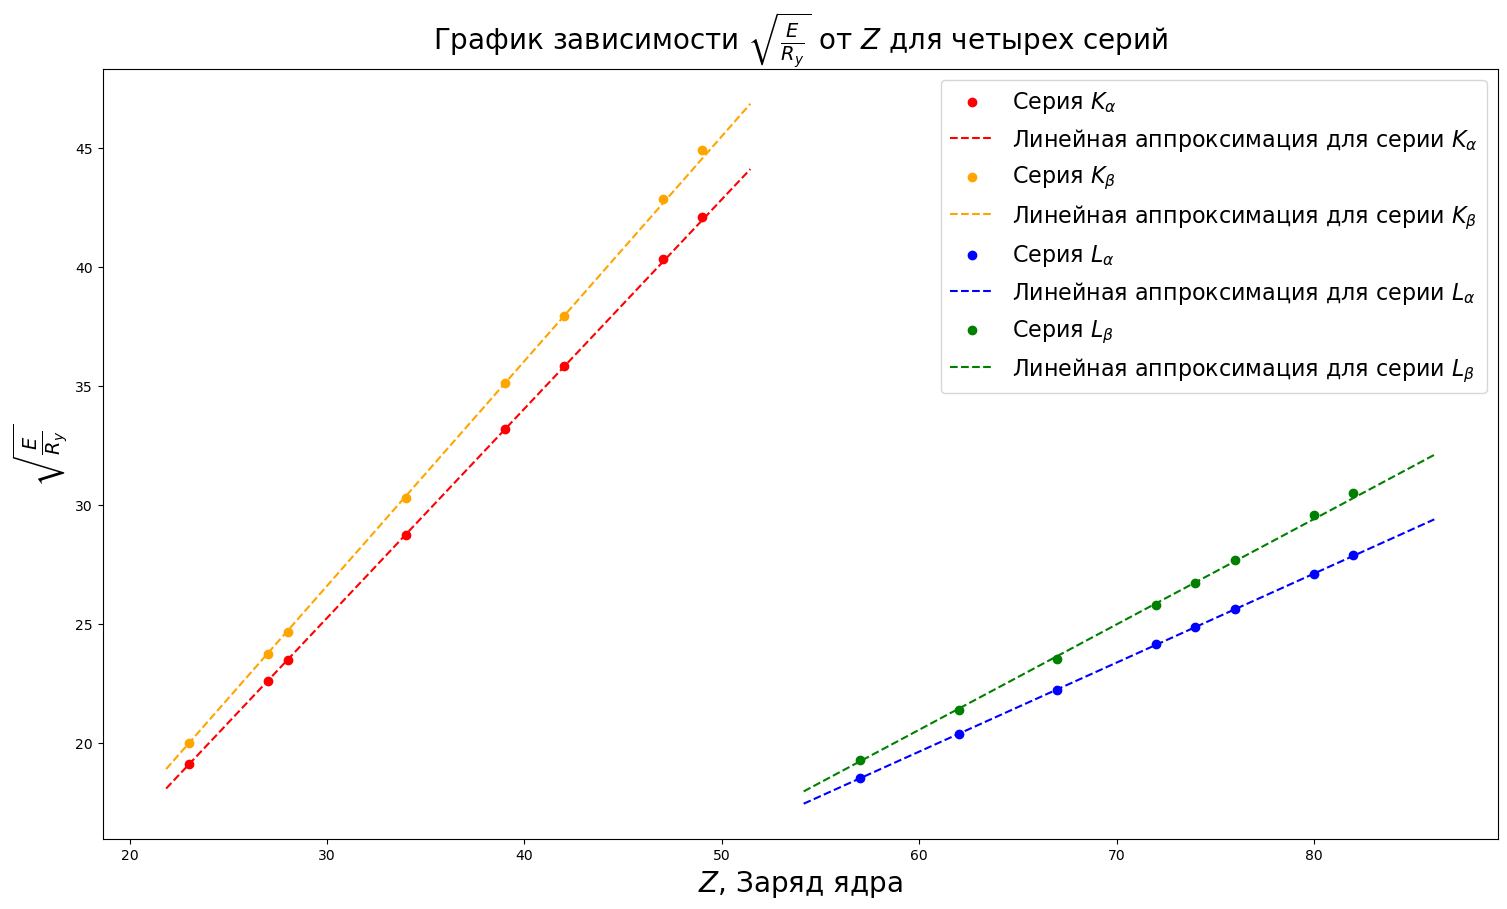
\includegraphics[width=1.02\linewidth]{График.png}
		\end{figure}

	\newpage

		Линейную аппроксимацию будем проводить взвешенным МНК: 

		\[k = \dfrac{\left<xy\right>' - \left<x\right>' \left<y\right>'}{\left<x^2\right>' - \left(\left<x\right>'\right)^2} \qquad
b = \left<y\right>' - k \left<x\right>',\]

где 

		\[\left<x\right>' = \dfrac{1}{W}\sum\limits_{i = 1}^n w_ix_i \qquad w_i = \dfrac{1}{\sigma_{y_i}} \qquad W = \sum\limits_{i = 1}^nw_i\]

А погрешности для $k$ и $b$:

		\[\sigma_k = \dfrac{1}{\sqrt{n}} \cdot \sqrt{\dfrac{\left<y^2\right>' - \left(\left<y\right>'\right)^2}{\left<x^2\right>' - \left(\left<x\right>'\right)^2} - k^2} \qquad \sigma_b = \sigma_k \cdot \sqrt{\left<x^2\right>' - \left(\left<x\right>'\right)^2}\]

		\begin{table}[!ht]
			\centering
			\begin{tabular}{|c|c|c|c|c|}
				\hline
				Спектральная линия & $k$ & $\sigma_k$ & $b$ & $\sigma_b$ \\
				\hline
				$K_{\alpha_{1, 2}}$ & 0.880 & 0.002 & -1.153 & 0.049 \\ 
				$K_{\beta_{1, 3}}$ & 0.945 & 0.004 & -1.759 & 0.093 \\ 
				$L_{\alpha_1}$ & 0.374 & 0.001 & -2.82 & 0.047 \\ 
				$L_{\beta_1}$ & 0.443 & 0.004 & -6.028 & 0.280 \\
				\hline
			\end{tabular}
			\caption{Результаты взвешенного МНК}
		\end{table}

		Из формулы:

		\[\hbar \omega = R_y \cdot (Z - \sigma)^2 \cdot \left(\dfrac{1}{n_1^2} - \dfrac{1}{n_2^2}\right)\]

		Получаем,  что постоянная экранирования равна $\sigma = -\frac{b}{k}$, а $k = \sqrt{\left(\frac{1}{n_1^2} - \frac{1}{n_2^2}\right)}$ для всех спектральных линий.  Сравним полученные данные с табличными:

		\begin{table}[!ht]
			\centering
			\begin{tabular}{|c|c|c|c|c|}
				\hline
				Спектральная линия & $\sigma_{\text{эксп}} = \frac{-b}{k}$ & $\sigma_{\text{теор}}$ & $k_{\text{эксп}}$ & $k_{\text{теор}} = \sqrt{\left(\frac{1}{n_1^2} - \frac{1}{n_2^2}\right)}$ \\
				\hline
				$K_{\alpha_{1, 2}}$ & $1.310 \pm 0.033$ & 1.0 & $0.880 \pm 0.002$ & 0.866 \\
				$K_{\beta_{1, 3}}$ & $1.862 \pm 0.028$ & 1.8 & $0.945 \pm 0.004$ & 0.943 \\
				$L_{\alpha_1}$ & $7.557 \pm 0.002$ & 7.4  & $0.374 \pm 0.001$ & 0.373 \\
				$L_{\beta_1}$ & $13.615 \pm 0.003$ & $\approx$ 14 & $0.443 \pm 0.004$ & 0.373 \\
				\hline
			\end{tabular}
			\caption{Сравнение полученных результатов с табличными}
		\end{table}

    \section*{Вывод}
    
    		\begin{enumerate}
    		
			\item В нашем эксперименте мы получили линейную зависимость корня из энергии характеристического излучения от заряда ядра - основную часть закона Мозли.  Причем,  как видно из графика с очень высокой точностью,  это связано с тем, что человеческий фактор не вносил почти никакую погрешность.
			
			\item Дополнительная часть закона Мозли говорит о том,  какие должны быть константы в этом законе,  как мы можем убедиться из таблицы выше,  измеренные константы близки к теоретическим ($L_{\beta_1}$ отдельным пунктом),  но не лежат в пределах погрешностей.  Это связано с тем,  что константы в законе - примерные (характеристические).
			
			\item Для $L_{\beta_1}$ коэффициент наклона достаточно сильно отличаются от табличного.  Это связано с тем,  что данная модель уже не подходит,  так как мы пытаемся описать многоэлектронную модель одночастичной.
    		
    		\end{enumerate}

\end{document}